\documentclass[aspectratio=169]{beamer}
\usetheme{Berlin}
\usepackage[utf8]{inputenc}
\usepackage[russian]{babel}
\usepackage{mhchem}
\usepackage{textpos} % for logo
\usepackage{amsmath} % for arg

\setbeamercovered{transparent} 

\newcommand{\CC}{C\nolinebreak\hspace{-.05em}\raisebox{.4ex}{\tiny\bf +}\nolinebreak\hspace{-.10em}\raisebox{.4ex}{\tiny\bf +}}
\def\CC{{C\nolinebreak[4]\hspace{-.05em}\raisebox{.4ex}{\tiny\bf ++}}} % define pretty C++

\graphicspath{ {../pics/} }
\title{Khnum: быстрая open-source программа для расчета метаболических потоков с использованием \ce{^{13}C}-углерода}
\author{Стешин Семен Сергеевич}
\institute{МГУ ВМК, кафедра математической кибернетики, 2020}
\date{}
\begin{document}
\begin{frame}[plain]
    \maketitle
    \begin{small}
    	 \begin{flushright}
    		Научный руководитель:\\
    		к.ф.м.н., доцент \\
    		Шуплецов М. С.
    	\end{flushright}
    \end{small}
   
\end{frame}

\section{Введение}
\begin{frame}{Анализ Метаболических Потоков}
\emph{Метаболический поток} --- внутриклеточная химическая реакция \pause

\emph{\ce{^{13}C}-Metabolic Flux Analysis} (\emph{\ce{^{13}C}-MFA}) --- метод измерения метаболических потоков
\end{frame}

\begin{frame}{Анализ Метаболических Потоков}
\includegraphics<1>[width=0.9\textwidth]{mfa_1.png}
\includegraphics<2>[width=0.9\textwidth]{mfa_2.png}
\includegraphics<3>[width=0.9\textwidth]{mfa_3.png}
\end{frame}

\begin{frame}{Анализ Метаболических Потоков}
	\centering
	\huge
	$f(v) = $\includegraphics<1->[trim=0 1cm 0 0]{calc.png} \vspace*{1cm}
	
	$\operatorname*{arg}_v f(v) \approx$ 
\includegraphics[trim=0 1cm 0 0]{mea.png}
\end{frame}

\begin{frame}{Анализ Метаболических Потоков}
	\begin{itemize}
	\uncover<1->{\item $\min_{\mathbf{v} \in U}{ } (\mathbf{x}_{mea} - \mathbf{x}_{calc}(\mathbf{v}))^T \times \mathbf{\Sigma}^{-1} \times (\mathbf{x}_{mea} - \mathbf{x}_{calc}(\mathbf{v}))$}
	\uncover<2->{\item Линейное программирование}
	\uncover<3->{\item Метод оптимизации}
	\uncover<4->{\item Конструирование графов}
	\uncover<5->{\item Создание СЛАУ}
	\uncover<6->{\item Решение СЛАУ}
	\uncover<7->{\item Статистика}
	\uncover<8->{\item Кластеризация результатов}
	\end{itemize}
\end{frame}



\begin{frame}{Программы для \ce{^{13}C}-MFA расчетов}
	\begin{itemize}
		\item \textbf{13CFLUX2}  
\includegraphics[height=\fontcharht\font`\B]{c.png}
		
		\item \textbf{Metran} 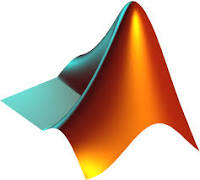
\includegraphics[height=\fontcharht\font`\B]{matlab.jpeg}
		
		\item \textbf{OpenFlux(2)} 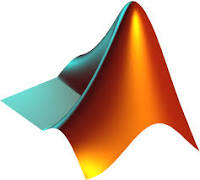
\includegraphics[height=\fontcharht\font`\B]{matlab.jpeg}
		
		\item \textbf{FluxPyt} 
\includegraphics[height=\fontcharht\font`\B]{python.jpeg}
		
		\item \textbf{mfapy} 
\includegraphics[height=\fontcharht\font`\B]{python.jpeg}
		
		\item \textbf{Sysmetab} 
\includegraphics[height=\fontcharht\font`\B]{Scilab_logo.png}
		
		\item \textbf{baMFA} 
\includegraphics[height=\fontcharht\font`\B]{python.jpeg}
		\item \textbf{iso2flux} 
\includegraphics[height=\fontcharht\font`\B]{python.jpeg}
		
		\item \textbf{Flux-P} 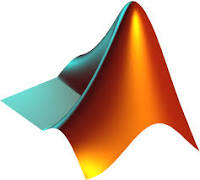
\includegraphics[height=\fontcharht\font`\B]{matlab.jpeg}
		\item \textbf{WUFlux} 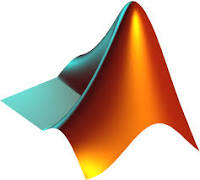
\includegraphics[height=\fontcharht\font`\B]{matlab.jpeg}
		\item \textbf{OpenMebius} 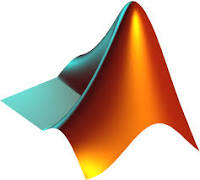
\includegraphics[height=\fontcharht\font`\B]{matlab.jpeg}
		\item \textbf{influx\_s} 
\includegraphics[height=\fontcharht\font`\B]{python.jpeg}
	\end{itemize}
\end{frame}

\section{Постановка задачи}
\begin{frame}{Постановка задачи}
	\begin{itemize}
		\item Написать эффективную программу для расчета \ce{^{13}C}-MFA на языке \CC{}
		\item Провести тестирование, сравнить скорость работы с существующими аналогами
	\end{itemize}
\end{frame}

\section{Khnum}
\begin{frame}{Программа Khnum}
Используемые библиотеки:
\begin{itemize}
	\item Eigen
	\item Alglib
	\item glpk
	\item Catch2
\end{itemize}

\texttt{https://github.com/SteshinSS/khnum}
\end{frame}

\begin{frame}{Замеры}
Метаболическая модель из 169 реакций

OpenFlux --- 35 минут

Khnum, один поток --- 22 секунды

Khnum, шестнадцать потоков --- 4 секунды
\end{frame}

\section{М-матрицы}
\begin{frame}{Матрицы метода}
\begin{columns}
	\begin{column}{0.5\textwidth}
		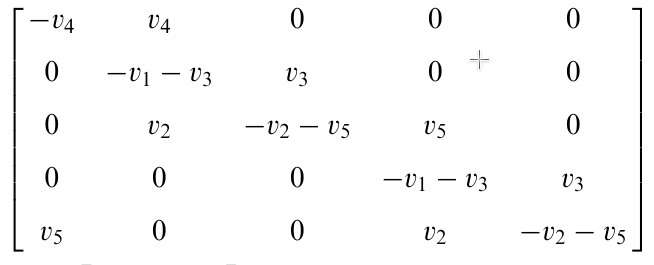
\includegraphics[width=\textwidth]{matrix.jpg}
	\end{column}
	\begin{column}{0.5\textwidth}
		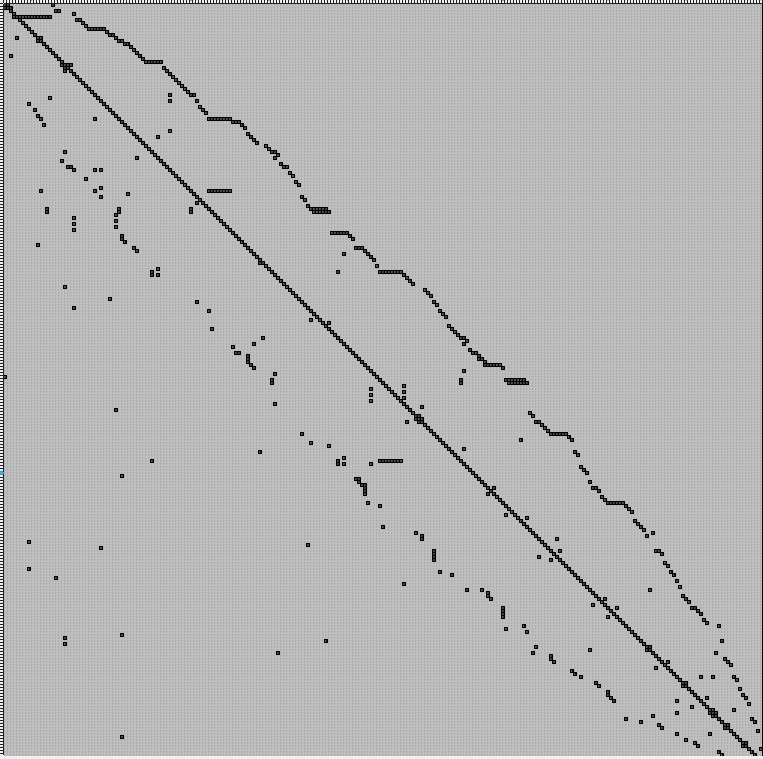
\includegraphics[width=0.8\textwidth]{sparse_matrix.jpg}
	\end{column}
\end{columns}
\end{frame}

\begin{frame}{М-матрицы}
\begin{block}{Определение М-матрицы (Ostrowsky, 1937)}
	Квадратная матрица $\mathbf{A} \in \mathbb{R}^{n \times n}$ называется \emph{М-матрицей}, если:
	\begin{enumerate}
		\item Ее диагональные элементы больше или равны нулю $a_{ii} \ge 0$, $i = j$
		\item Ее внедиагональные элементы меньше или равны нулю $a_{ij} \le 0$, $i \neq j$
		\item Матрицу $\mathbf{A}$ можно представить в виде: $\mathbf{A} = s\mathbf{I} - \mathbf{B}$, где $s > 0$, $\mathbf{B} \ge 0$, $s > \rho(\mathbf{B})$, где $\rho(\mathbf{B})$ --- спектральный радиус $\mathbf{B}$
	\end{enumerate}
\end{block}

\end{frame}

\begin{frame}{М-матрицы}
\begin{block}{Критерий М-матриц (Fiedler, Ptak, 1962)}
	Квадратная матрица является М-матрицей тогда и только тогда, когда она невырожденная и все вещественные собственные значения ее главных миноров больше или равны нулю. 
\end{block}
\end{frame}

\begin{frame}{М-матрицы}
\begin{block}{Теорема кругов (Гершгорин, 1931)}
	Пусть $\mathbf{A} \in \mathbb{C}^{n \times n}$ --- комплексная матрица. Пусть $R_i = \sum_{i \neq j} |a_{ij}|$ --- сумма модулей внедиагональных элементов $i$ строки. Кругом Гершгорина назовем замкнутый круг $D(a_{ii}, R_i)$ с центром в $a_{ii}$ и радиусом $R_i$. Тогда каждое собственное значение матрицы $\mathbf{A}$ лежит хотя бы в одном круге Гершгорина. 
\end{block}
\end{frame}

\begin{frame}{М-матрицы}
\begin{block}{Теорема-результат}
	Матрица коэффициентов MFA-систем, взятая со знаком минус, является М-матрицей.
\end{block}
\end{frame}

\section{ILU-разложение}
\begin{frame}{ILU-разложение}
\begin{block}{Определение ILU-разложения (Meijerink, van der Vorst, 1977)}
	Пусть $\mathbf{A} \in \mathbb{R}^{n \times n}$ --- разреженная матрица. Определим для нее \emph{разреженную структуру} $S = \{(i, j) | a_{ij} \neq 0\} \cup \{(i,i)\}$ состоящую из всех координат ненулевых элементов и всех диагональных координат. Назовем \emph{ILU-разложением} разложение вида $\mathbf{A} = \mathbf{L}\mathbf{U} - \mathbf{R}$, где
	\begin{itemize}
		\item $\mathbf{L} \in \mathbb{R}^{n \times n}$ --- нижнетреугольная матрица
		\item $\mathbf{U} \in \mathbb{R}^{n \times n}$ --- верхнетреугольная матрица
		\item $\mathbf{L}, \mathbf{U}$ равны нулю вне разреженной структуры: $\mathbf{L}_{ij} = \mathbf{U}_{ij} = 0 \forall (i, j) \notin S$
		\item $\mathbf{R} \in \mathbb{R}^{n \times n}$ равна нулю в разреженной структуре: $\mathbf{R}_{ij} = 0 \forall (i, j) \in S$
	\end{itemize}
\end{block}
\end{frame}

\begin{frame}{Замеры}
М-матрица $253 \times 253$
\begin{itemize}
	\item BiCGSTAB + ILU
	\item BiCGSTAB + Diag
	\item LU (Partial Pivoting)
	\item SuperLU + COLAMD
\end{itemize}
\begin{table}[b]
	\centering
	\caption{Сравнение методов. Время в микросекундах\label{methods_benchmark}}
	\begin{tabular}{c|c|c|c}
		\hline
		BiCGSTAB + ILU & BiCGSTAB + Diag & DenseLU & SparseLU\\
		\hline
		125 & 986 & 645 & 174\\
	\end{tabular}
\end{table}
\end{frame}

\section{Модель Леонтьева}
\begin{frame}{Продуктивная матрица}
\begin{block}{Определение продуктивной матрицы (Леонтьев, 1928)}
	Квадратная вещественная матрица $\mathbf{A} \in \mathbb{R}^{n \times n}$ называется продуктивной, если
	\begin{itemize}
		\item $a_{ij} \leq 0, \forall i \neq j$
		\item $\exists x \geq 0 : Ax > 0$
	\end{itemize}
\end{block}
\end{frame}

\begin{frame}{Сравнение моделей}
\begin{columns}[T]
	\column{0.5\textwidth}
	\begin{itemize}
		\item Есть несколько отраслей
		\item Они используют ресурсы друг друга, чтобы производить ресурсы
		\item Экономика сильна
	\end{itemize}

	\column{0.5\textwidth}
	\begin{itemize}
		\item Есть несколько химических реакций
		\item Они используют метаболиты друг друга, чтобы производить метаболиты
		\item Клетка жива
	\end{itemize}
\end{columns}
\end{frame}

\begin{frame}{Ряд Неймана}
\begin{block}{Обращение М-матрицы (F. Waugh, 1950)}
	Пусть $\mathbf{A} = c\mathbf{I} - \mathbf{B}$ --- невырожденная М-матрица. Тогда $\mathbf{A} = \sum_{k = 0}^{\infty} \frac{\mathbf{A}^k}{c^{k+1}}$, причем ряд абсолютно сходится.
\end{block}
\end{frame}

\section{Полученные результаты}
\begin{frame}{Полученные результаты}
	\begin{itemize}
		\item Написана эффективная открытая программа Khnum для проведения \ce{^{13}C}-MFA расчетов.
		\item Проведено сравнение с аналогами.
		\item Доказана принадлежность матрицы коэффициентов СЛАУ к классу М-матриц. Это позволило использовать специальный предобуславливатель на основе ILU-разложения.
		\item Проведено сравнение нескольких численных методов для СЛАУ \\ Показано, что численные методы с ILU-предобуславливателем\\ работают быстрее всего.
	\end{itemize}
\end{frame}

\section*{}
\begin{frame}
	\centering
	\Large
	Спасибо за внимание
\end{frame}
\end{document}
